\chapter{Experiments: Random Geometric Graphs}

\textcolor{red}{
  Perhaps the first word that springs to mind when thinking about spatial
constraints to graph, is ``space''. It is only natural that we begin with the
simplest spatial network there is -- the random geometric graph, of which the
only spatial constraint is that the vertices of the graph are placed in some
underlying metric space.
}

\textcolor{red}{
  Random geometric graph is the simplest spatial network, where $N$ nodes are
placed randomly in some metric space. The specific probability distribution is
just a uniform distribution in an underlying Euclidean space $[0, N)^d$, where
$d$ is the dimensionality of the volume. Nodes have some neighborhood within a
radius of $r$, of which nodes inside this radius will be connected by an edge.
}

\textcolor{red}{
  Perhaps talk about similar models, such as Waxman and Erdos-Renyi. They should
have been introduced in the background chapter, so we can refer to them
here. The Erdos-Renyi is perhaps the closest spatial model to the echo state
network, and the Waxman network is a generalized random geometric graph with a
slight modification for node connectivity, i.e. a probabilistic connection
function.
}

% (TODO): t!
\begin{figure}[t]
  \centering
  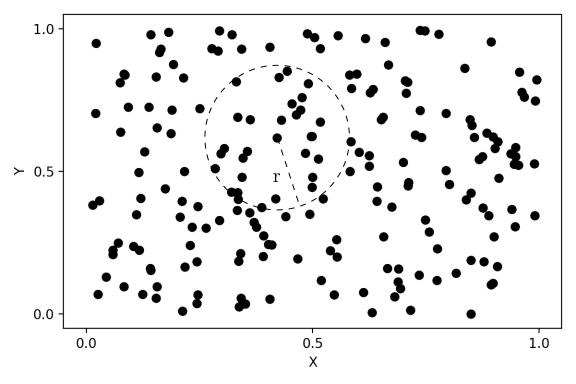
\includegraphics[width=3.5in]{figures/RGG-example.png}
  \caption{
    Example vertices drawn to generate a random geometric graph embedded in a
two-dimensional Euclidean space. The neighborhood radius $r$ of a single node is
shown.
  }
  \label{fig:rgg-example}
\end{figure}

\section{Methodology}

% (TODO): Section references should be added as sections are added and
% completed.
\textcolor{red}{
  \textbf{Methodology:} We use fully connected graphs. I.e. distance r of
infinity. We use 3d networks by default, but this is investigated further. We
introduce distance functions to the model, of which used ones are $1/d$, $1/d^2$
and $1/d^3$. So they are connected if $d(x, y, z) < r$, where $d(x, y, z) =
\norm{x-y}_{2} = \sqrt{\sum_{i=1}^{d}{(x_{i}-y_{i})^2}}$, and $r = \infty$. The
implementation is a standard echo state network from the methodology chapter
where weights are determined by the scheme above.
}

\section{Size of the Underlying Volume}

\subsection{Synopsis}

\textcolor{red}{
  A natural first question when considering random geometric graphs is that of
the underlying space. The behavior of the ``echo state network'' that we create
will obviously be affected by the magnitude of the weights we create between the
hidden nodes.
}

\textcolor{red}{
  The most interesting metric for the resulting matrices is of course the
spectral radius, i.e. the largest eigenvalue, as this governs dynamics, and a
very high one may cause unbounded deviation from initial states, even though the
tanh activation bounds the actual activations. How does the spectral radius
relate to the performance of our network, and can this be related to previous
work?
}

\subsection{Results and Discussion}

% (TODO): t!
\begin{figure*}[t!]
  \centering
  \begin{subfigure}{.49\textwidth}
    \centering
    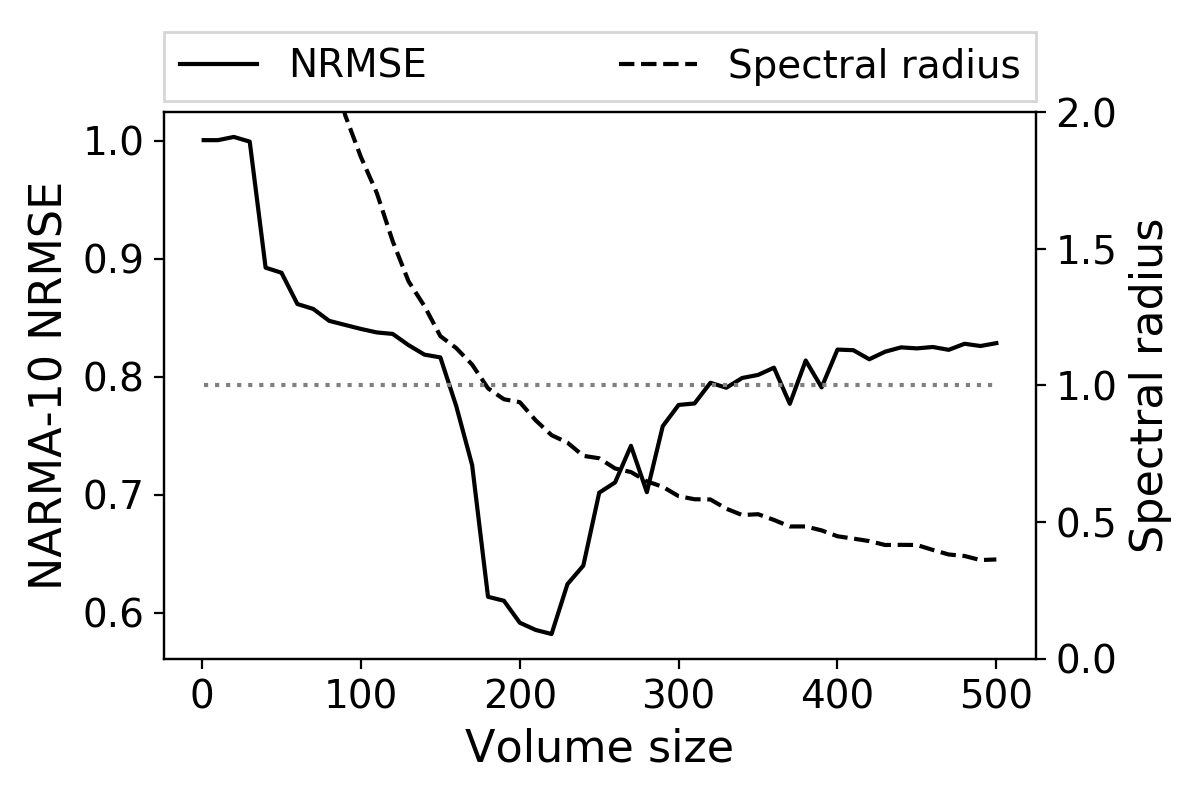
\includegraphics[width=1.0\linewidth]{figures/RGG-volume-size-inv.png}
    \caption{}
    \label{fig:size-graph-volume-a}
  \end{subfigure}
  \begin{subfigure}{.49\textwidth}
    \centering
    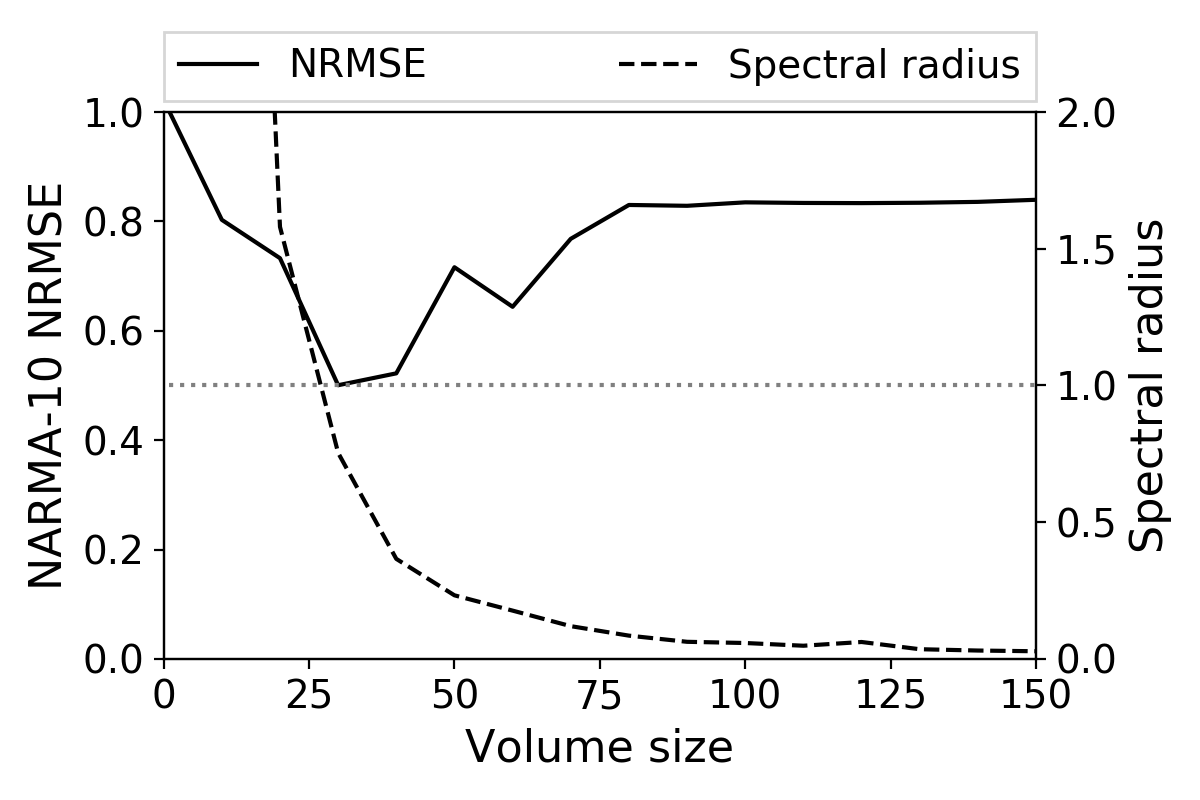
\includegraphics[width=1.0\linewidth]{figures/RGG-volume-size-inv-squared.png}
    \caption{}
    \label{fig:size-graph-volume-b}
  \end{subfigure}
  \caption{
    Spectral radius and performance of generated random geometric graphs of size
$N = 100$, as a function of the size of the underlying volume. Illustrated is
node coupling using two different distance functions: $1/d$ (a) and $1/d^2$ (b).
  }
  \label{fig:size-graph-volume}
\end{figure*}

\textcolor{red}{
  We immediately see that using a volume of size 1x1x1 is useless, as this would
produce nodes that are very close. Nodes that are too close will drive the 1/d
function through the roof (as the weights will potentially be quite large), and
we will immediately saturate $tanh$ activations in the network.
}

\textcolor{red}{
  Figure \ref{fig:size-graph-volume} illustrates the point by scaling the size
of the underlying volume. The volume goes from 1x1x1 through the sizes in the
plot as NxNxN where N is the ``volume size''. We plot both the NRMSE and
spectral radius of the resulting w_res of the echo state network, and can
clearly pinpoint a similar result to that of the literature: a spectral radius
$\rho < 1$, but not too small, is favored. We should also specify that the
spectral radius is the absolute value of the largest eigenvector, which controls
the dynamics of the system, see ``On the quantifications..'' paper, see
Verstraeten et al.
}

\textcolor{red}{
  Performance-wise we see that both distance functions achieve an NRMSE a little
bit below 0.6, which is worse than what a shift register would achieve. Thus, we
are nowhere close to the echo state network, and a spatial constraint like this
by itself seems to induce a big performance penalty/increase in error.
}

\textcolor{red}{
  For further experiments, we can remedy this initial issue by scaling directly
by the spectral radius, which fixes the problem. Scaling by the spectral radius
is done by multiplying the weight by a scalar, which would be equivalent to
scaling underlying volume with a scalar. This is relevant for physical mediums,
as what we are seeing in practice is that distance function in conjunction with
the size of the space is quite relevant, otherwise we dip to either side of
Figure \ref{fig:size-graph-volume}.
}

\subsection{Summary}

\textcolor{red}{
  The summary of what we see is that if we were to design a reservoir by
modeling it after a random geometric graph, we would have to think about the
size of the space we are using, especially if the distance function that must be
used is fixed by the laws of physics.
}

\section{Choice of Distance Function}

\subsection{Synopsis}

\textcolor{red}{
  Different systems may exhibit different characteristics. For example flatspin
uses couplings of $1/d^3$. Not necessarily directly comparable, but it is an
interesting problem from a theoretical standpoint.
}

\textcolor{red}{
  In this section we compare the distance functions $1/d$, $1/d^2$ and $1/d^3$,
and also see how they compare to the standard echo state network. We also look a
little deeper into why these functions seem to be unable to reach the level of
the ESN by looking at short-term memory capacity.
}

\textcolor{red}{
  \textbf{Methodology}: Here we are using what we figured out in the previous
section, and scale the spectral radius directly. We set the spectral radius to
0.9, and use the same input scheme again, which is uniform sampling in the
interval [-0.5, 0.5].
}

\subsection{Results and Discussion}

% (TODO): t!
\begin{figure*}[t]
  \centering
  \begin{subfigure}{.49\textwidth}
    \centering
    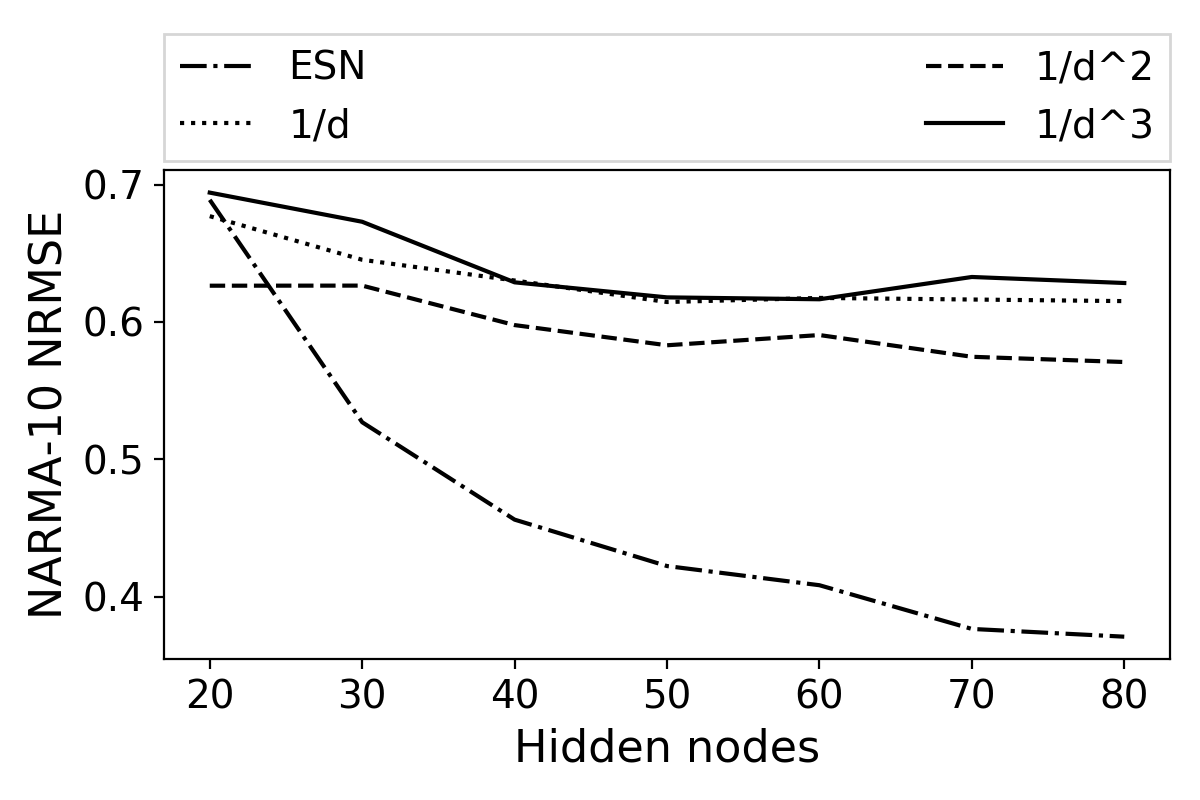
\includegraphics[width=1.0\linewidth]{figures/RGG-dist-performance-mean.png}
    \caption{}
    \label{fig:dist-performance-a}
  \end{subfigure}
  \begin{subfigure}{.49\textwidth}
    \centering
    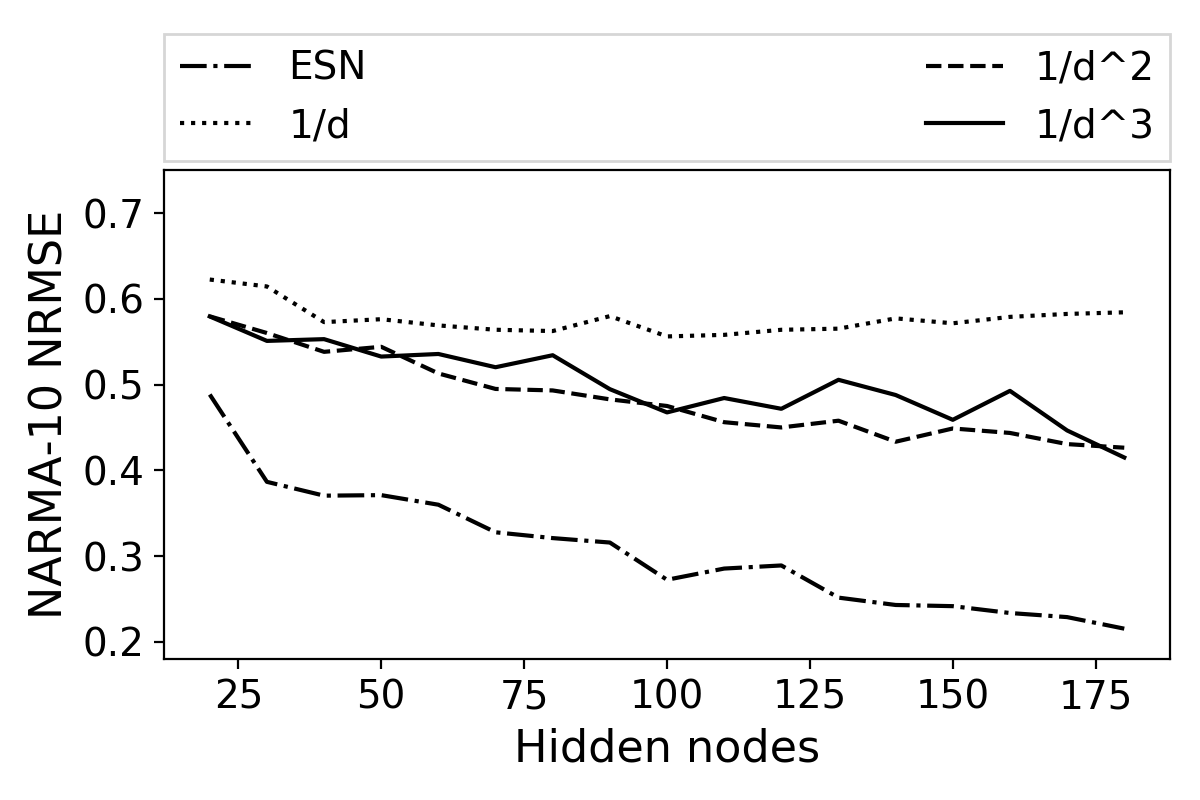
\includegraphics[width=1.0\linewidth]{figures/RGG-dist-performance-min.png}
    \caption{}
    \label{fig:dist-performance-b}
  \end{subfigure}
  \caption{
    NRMSE on the NARMA-10 task with use of different distance functions to
generate connection weights. Plots shown are the mean (a) and minimum (b) error
aggregations over 10 runs per individual parameter setup. Distance functions are
compared to the standard echo state network.
  }
  \label{fig:dist-performance}
\end{figure*}

% (TODO): Consider 3d plots for hidden nodes.
% (TODO): t!
\begin{figure*}[t]
  \centering
  \begin{subfigure}{.49\textwidth}
    \centering
    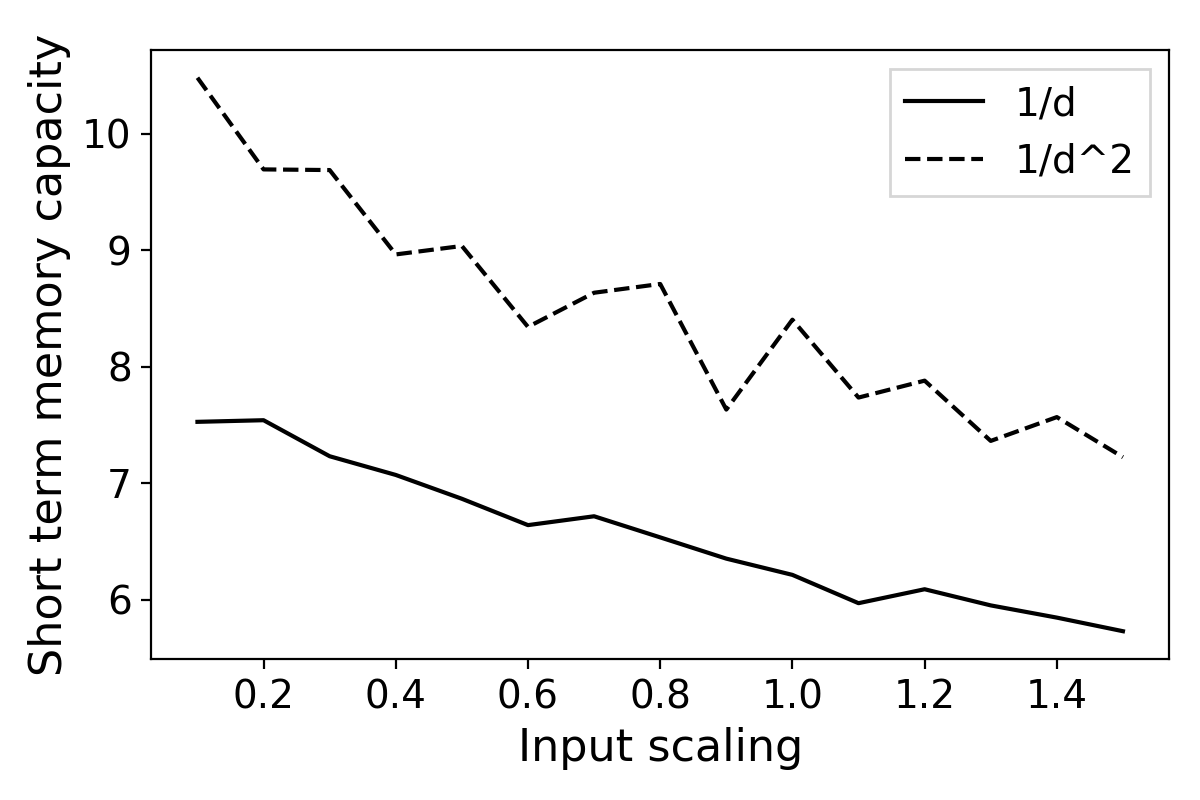
\includegraphics[width=1.0\linewidth]{figures/RGG-dist-mc.png}
    \caption{}
    \label{fig:dist-performance-is-a}
  \end{subfigure}
  \begin{subfigure}{.49\textwidth}
    \centering
    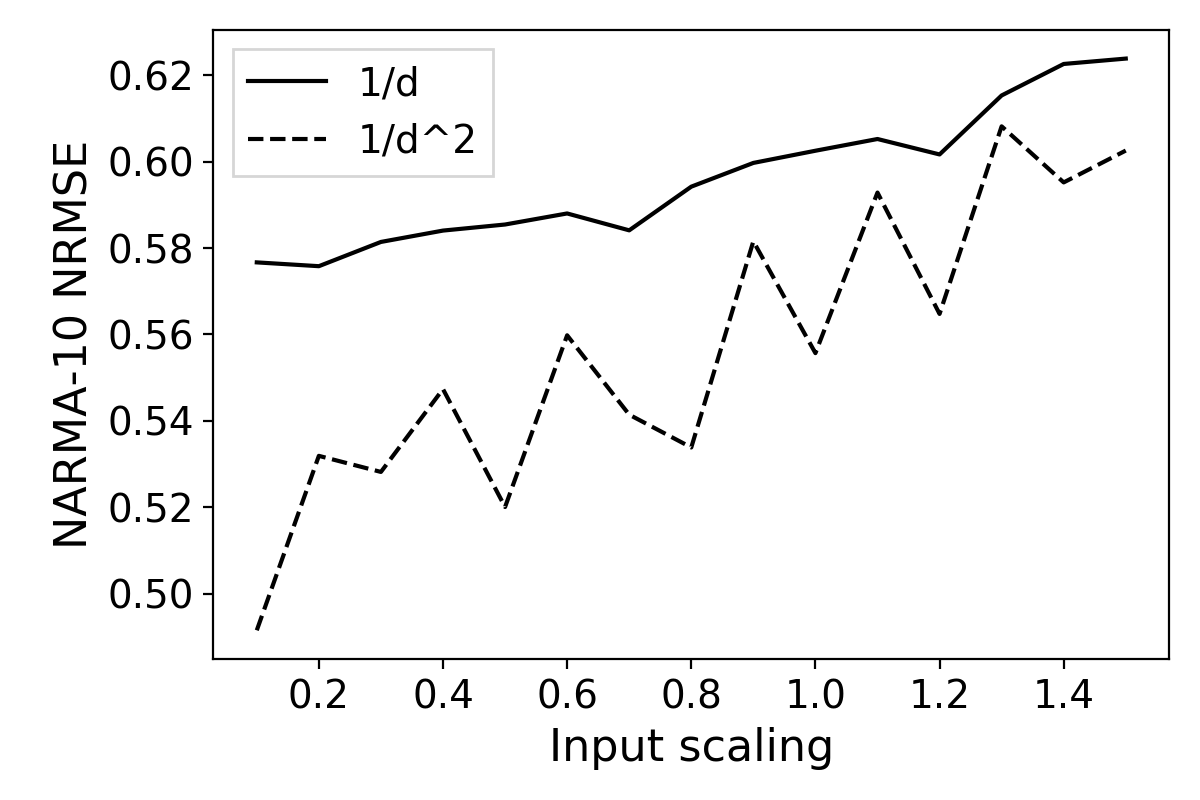
\includegraphics[width=1.0\linewidth]{figures/RGG-dist-performance-is.png}
    \caption{}
    \label{fig:dist-performance-is-b}
  \end{subfigure}
  \caption{
    Effect of input scaling on reservoirs generated as random geometric
graphs. There is a correlation between the short-term memory capacity of the
reservoirs (a), and error rates for the NARMA-10 task (b).
  }
  \label{fig:dist-performance-is}
\end{figure*}

\textcolor{red}{
  We see that all distance functions are quite far away from the echo state
network, as was established earlier. We also notice that they seem to be quite
unstable compared to the ESN in generation, especially $1/d^3$ has a bad mean
over the runs, but a min that is on par with $1/d^2$. Why is not immediately
clear, but will be resolved in the next section with additions of signed and
directed edges.
}

\textcolor{red}{
  We see that all the distance functions see a significant improvement from
increasing the size of the reservoir, but not as great as that of the echo state
network. Note that this is without exhausting the parameters that are usually
swept: input scaling and spectral radius. In a further experiment, we look at
why these networks are significantly worse than ESNs by choosing the $1/d^2$
distance function, and looking and something that intuitively seems to be the
cause: short-term memory, which is shown in Figure
\ref{fig:dist-performance-is}.
}

\textcolor{red}{
  A thought that may arise when looking at this, is that the random geometric
graph reservoirs will never reach the performance of a delay line, even with
bigger reservoirs. This indicates that their memory capacity is perhaps not up
to par, which is further illustrated in Figure
\ref{fig:dist-performance-is}. The setup for this experiment was 10 runs, where
the short-term memory is the max value, and the NRMSE is the min value for the
reservoirs generated.
}

\textcolor{red}{
  Thus, we see that we may increase the performance of RGG reservoirs by using
the commonly swept input scaling parameter to exchange nonlinear dynamics for
memory. Reservoirs seem to get significantly better once we reach the required
memory capacity of 10, but is still slightly behind the echo state network when
comparing e.g. the 80 node network in Figure \ref{fig:dist-performance-is-b} to
that of the echo state network of size 80 nodes in Figure
\ref{fig:dist-performance}
}

\subsection{Summary}

\textcolor{red}{
  We see that some distance functions seem to perform better, namely $1/d^2$
seems to be both the best performing, while also being quite stable. We also see
that the default performance of the random geometric graphs for $1/d^2$ suffer
from a low short-term memory capacity, which, in the case of NARMA-10, may be
remedied by lowering the input scaling to wash older inputs out slower.
}

\section{Restoring Echo State Network Performance}

\subsection{Synopsis}

\subsection{Results and Discussion}

\subsection{Summary}

\section{Reservoir Weight Distributions}

\subsection{Synopsis}

Reciprocal normal distribution. Cite common ones in practice from practical
applications paper.

\subsection{Results and Discussion}

\subsection{Summary}

\section{Dimensionality of the Underlying Space}

\subsection{Synopsis}

Does it matter if we choose xy, xyz, xyzw?

\subsection{Results and Discussion}

\subsection{Summary}

\section{Conclusions}

\textcolor{red}{
  We have investigated imposing the simplest type of spatial restriction onto
echo state networks, and found that they by default will worsen significantly by
default. Care must be taken to ensure that the spacing between nodes will result
in node interactions that induce reservoir dynamics that are suitable for the
task at hand. This is especially important in physical reservoir computing where
the distance between nodes decides their coupling, and it can not be changed
after-the-fact.
}

% (TODO): Look more into this if found _why_ this causes this improvement,
% concretely.
\textcolor{red}{
  Further we investigated why the spatial restrictions worsened the networks
significantly, arriving at some interesting conclusions regarding flow of
information.
}

\textcolor{red}{
  Highlight the important discoveries in this chapter that lead well into the
next chapter. We would like to highlight two key discoveries: \textbf{(1)} the
fact that there are other weighting distribution schemes that work just as well
as uniform and normal, here we have discovered something that resembles the
reciprocal normal distribution using $1/d$, $1/d^2$ etc. And \textbf{(2)} that
reservoirs worsen significantly if there is no inherent flow of information,
which we in this case restored by introducing signedness and directedness to the
reservoir edges. These discoveries are important springboards into the next
chapter.
}


%%% Local Variables:
%%% mode: latex
%%% TeX-master: "../thesis"
%%% End:
